\protect\hypertarget{c1}{}{}


\section{Resonance}\label{resonance}

Resonance in AC circuits implies a special frequency determined by the
values of the
\href{http://hyperphysics.phy-astr.gsu.edu/hbase/electric/acres.html\#c1}{resistance}
,
\href{http://hyperphysics.phy-astr.gsu.edu/hbase/electric/accap.html\#c1}{capacitance}
, and
\href{http://hyperphysics.phy-astr.gsu.edu/hbase/electric/acind.html\#c1}{inductance}
. For
\href{http://hyperphysics.phy-astr.gsu.edu/hbase/electric/serres.html\#c2}{series
resonance} the condition of resonance is straightforward and it is
characterized by minimum impedance and zero phase.
\href{http://hyperphysics.phy-astr.gsu.edu/hbase/electric/parres.html\#c1}{Parallel
resonance} , which is more common in electronic practice, requires a
more careful definition.


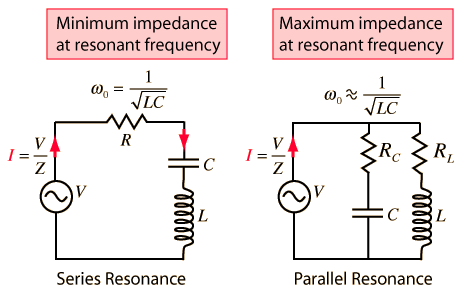
\includegraphics{./resonant-rlc-circuits_files/acres.png}

\protect\hypertarget{c2}{}{}

\section{Series Resonance}\label{series-resonance}

The
\href{http://hyperphysics.phy-astr.gsu.edu/hbase/electric/serres.html\#c1}{resonance}
of a series
\href{http://hyperphysics.phy-astr.gsu.edu/hbase/electric/rlcser.html\#c1}{RLC
circuit} occurs when the
\href{http://hyperphysics.phy-astr.gsu.edu/hbase/electric/acind.html\#c1}{inductive}
and
\href{http://hyperphysics.phy-astr.gsu.edu/hbase/electric/accap.html\#c1}{capacitive}
reactances are equal in magnitude but cancel each other because they are
180 degrees apart in
\href{http://hyperphysics.phy-astr.gsu.edu/hbase/electric/phase.html\#c1}{phase}.
The sharp minimum in
\href{http://hyperphysics.phy-astr.gsu.edu/hbase/electric/imped.html\#c1}{impedance}
which occurs is useful in tuning applications. The
\href{http://hyperphysics.phy-astr.gsu.edu/hbase/electric/serres.html\#c3}{sharpness}
of the minimum depends on the value of R and is characterized by the
``Q'' of the circuit.


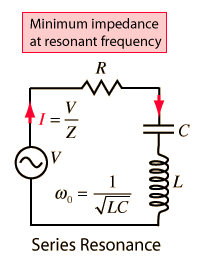
\includegraphics{./resonant-rlc-circuits_files/acres2.png}\strut

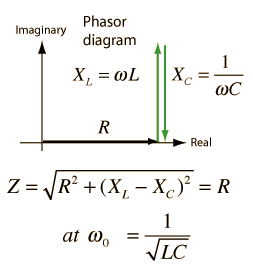
\includegraphics{./resonant-rlc-circuits_files/acres3.png}


\href{http://hyperphysics.phy-astr.gsu.edu/hbase/electric/rlcser.html\#c1}{Detailed
expressions} 
\href{http://hyperphysics.phy-astr.gsu.edu/hbase/electric/rlcser.html\#c2}{Calculation}\tabularnewline

\href{http://hyperphysics.phy-astr.gsu.edu/hbase/hframe.html}{Index}\\[2\baselineskip]\href{http://hyperphysics.phy-astr.gsu.edu/hbase/electric/accircon.html\#c1}{AC
Circuits}\strut

\href{http://hyperphysics.phy-astr.gsu.edu/hbase/hph.html}{HyperPhysics}*****\href{http://hyperphysics.phy-astr.gsu.edu/hbase/emcon.html\#emcon}{Electricity
and Magnetism} \emph{R Nave}

\protect\hypertarget{c3}{}{}

\section{Selectivity and Q of a
Circuit}\label{selectivity-and-q-of-a-circuit}

Resonant circuits are used to respond selectively to signals of a given
frequency while discriminating against signals of different frequencies.
If the response of the circuit is more narrowly peaked around the chosen
frequency, we say that the circuit has higher ``selectivity''. A
``quality factor'' Q, as described below, is a measure of that
selectivity, and we speak of a circuit having a ``high Q'' if it is more
narrowly selective.

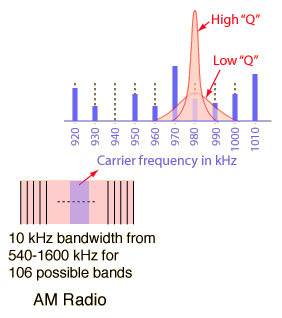
\includegraphics{./resonant-rlc-circuits_files/qamrad.png}\strut
An example of the application of resonant circuits is the selection of
\href{http://hyperphysics.phy-astr.gsu.edu/hbase/audio/radio.html\#c1}{AM
radio} stations by the radio receiver. The selectivity of the tuning
must be high enough to discriminate strongly against stations above and
below in carrier frequency, but not so high as to discriminate against
the
"\href{http://hyperphysics.phy-astr.gsu.edu/hbase/audio/sumdif.html\#c2}{sidebands}"
created by the imposition of the signal by amplitude modulation.\strut

The selectivity of a circuit is dependent upon the amount of resistance
in the circuit. The variations on a
\href{http://hyperphysics.phy-astr.gsu.edu/hbase/electric/serres.html\#c2}{series
resonant circuit} at right follow an example in Serway \& Beichner. The
smaller the resistance, the higher the ``Q'' for given values of L and
C. The
\href{http://hyperphysics.phy-astr.gsu.edu/hbase/electric/parres.html\#c1}{parallel
resonant circuit} is more commonly used in electronics, but the algebra
necessary to characterize the resonance is much more involved.\strut
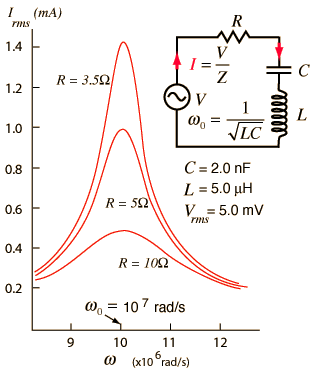
\includegraphics{./resonant-rlc-circuits_files/qresi.png}\strut

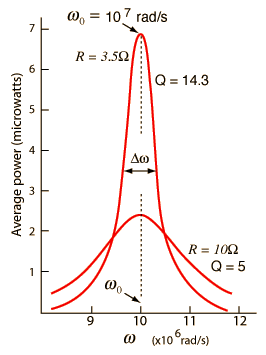
\includegraphics{./resonant-rlc-circuits_files/qpow.png}\strut
Using the same circuit parameters, the illustration at left shows the
\href{http://hyperphysics.phy-astr.gsu.edu/hbase/electric/serres.html\#c4}{power
dissipated} in the circuit as a function of frequency. Since this power
depends upon the square of the current, these resonant curves appear
steeper and narrower than the resonance peaks for current above.

The quality factor Q is defined by\\

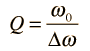
\includegraphics{./resonant-rlc-circuits_files/qdef.png}

where $\delta \omega$ is the width of the resonant power curve at half maximum.\strut

Since that width turns out to be $\delta \omega =R/L$, the value of Q can also be
expressed as

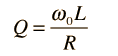
\includegraphics{./resonant-rlc-circuits_files/qdef2.png}

The Q is a commonly used parameter in electronics, with values usually
in the range of Q=10 to 100 for circuit applications.\strut
\href{http://hyperphysics.phy-astr.gsu.edu/hbase/hframe.html}{Index}\\[2\baselineskip]\href{http://hyperphysics.phy-astr.gsu.edu/hbase/electric/accircon.html\#c1}{AC
Circuits}\\[2\baselineskip]Reference\\
\href{http://hyperphysics.phy-astr.gsu.edu/hbase/electric/eleref.html\#c1}{Serway
\& Beichner}\\
Ch 33\strut

\href{http://hyperphysics.phy-astr.gsu.edu/hbase/hph.html}{HyperPhysics}*****\href{http://hyperphysics.phy-astr.gsu.edu/hbase/emcon.html\#emcon}{Electricity
and Magnetism}  \emph{R Nave}

\href{Javascript:history.go(-1)}{Go Back}\strut


\protect\hypertarget{c4}{}{}

\section{Power in a Series Resonant
Circuit}\label{power-in-a-series-resonant-circuit}

The average power dissipated in a
\href{http://hyperphysics.phy-astr.gsu.edu/hbase/electric/serres.html\#c2}{series
resonant circuit} can be expressed in terms of the
\href{http://hyperphysics.phy-astr.gsu.edu/hbase/electric/acres.html\#c2}{rms}
voltage and current as follows:

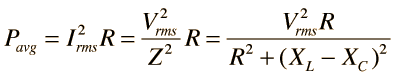
\includegraphics{./resonant-rlc-circuits_files/pser.png}

Using the forms of the inductive reactance and capacitive reactance, the
term involving them can be expressed in terms of the frequency.

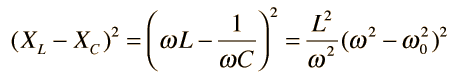
\includegraphics{./resonant-rlc-circuits_files/pser2.png}

where use has been made of the resonant frequency expression

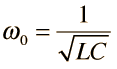
\includegraphics{./resonant-rlc-circuits_files/pser3.png}

Substitution now gives the expression for average power as a function of
frequency.

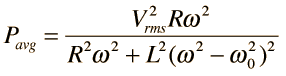
\includegraphics{./resonant-rlc-circuits_files/pser4.png}

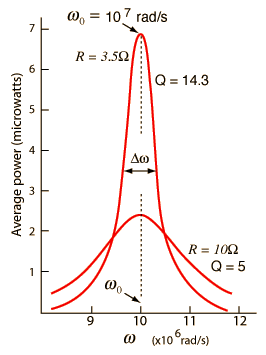
\includegraphics{./resonant-rlc-circuits_files/qpow.png}\strut

This power distribution is plotted at left using the same circuit
parameters as were used in the example on the
\href{http://hyperphysics.phy-astr.gsu.edu/hbase/electric/serres.html\#c3}{Q
factor} of the series resonant circuit

The average power at resonance is just\\

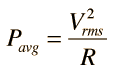
\includegraphics{./resonant-rlc-circuits_files/pser5.png}

since at the resonant frequency $\omega_0$ the reactive parts
cancel so that the circuit appears as just the resistance R.\strut

\href{http://hyperphysics.phy-astr.gsu.edu/hbase/hframe.html}{Index}\\[2\baselineskip]\href{http://hyperphysics.phy-astr.gsu.edu/hbase/electric/accircon.html\#c1}{AC
Circuits}\\[2\baselineskip]Reference\\
\href{http://hyperphysics.phy-astr.gsu.edu/hbase/electric/eleref.html\#c1}{Serway
\& Beichner}\\
Ch 33\strut

\href{http://hyperphysics.phy-astr.gsu.edu/hbase/hph.html}{HyperPhysics}*****\href{http://hyperphysics.phy-astr.gsu.edu/hbase/emcon.html\#emcon}{Electricity
and Magnetism} \emph{R Nave}

